\section*{OSN 17 Понятие анонимности пользователя в сети. Идентификаторы пользователя в сети на разных уровнях (устройства, ОС, ПО). Подходы к деанонимизациии, способы защиты. Концепция анонимных сетей (Mix и Tor). Луковая маршрутизация. Виды атак на анонимные сети.}

\subsubsection{Анонимность пользователя в сети}

\begin{itemize}
    \item Защита от наблюдения со стороны Интернет-провайдера (а также тех, кто его контролирует):
    – цензура
    
    – контекстная реклама
    
    – осуществление общественной, гражданской или политической деятельности
    \item Защита от наблюдения со стороны посещаемого ресурса    
\end{itemize}

\begin{itemize}
    \item Социальная анонимность – распространение (осознанное/неосознанное) в сети
персональной информации самим пользователем
    \item Техническая анонимность:
    
    – контроль за хранением и безопасностью персональных данных посредством специальных технических средств (как программных, так и аппаратных)
    
    – минимизация возможности утечки персональных данных
\end{itemize}

\textbf{Анонимность субъекта} (anonymity) -- злоумышленник не может с достаточной степенью точности идентифицировать субъект в рамках некоторого множества субъектов со схожим
набором атрибутов.

\textbf{Виды анонимности}:
\begin{itemize}
    \item Анонимность отправителя -- ни получатель сообщения, ни атакующий, наблюдающий за некоторым участком сети (между отправителем и получателем), не могут установить отправителя сообщения
    \item Анонимность получателя -- атакующий, наблюдающий за некоторым участком сети, не может установить получателя сообщения
    \item Анонимность взаимодействия -- атакующий, наблюдающий за некоторым участком сети, не может достоверно установить, от какого отправителя и какому получателю доставляется конкретное сообщение
    \item $K$-анонимность: пользователь сети не может на практике отличаться, по крайней мере, от $(K - 1)$ других пользователей сети, когда $K$ достаточно большое. Вводится для количественной оценки уровня анонимности, предоставляемого системой анонимизации отдельному пользователю
\end{itemize}

\subsubsection{Идентификаторы пользователя в сети}

Устройство пользователя:
\begin{itemize}
    \item \textit{Адресные признаки устройства}: MAC-адрес сетевого интерфейса, IP-адрес, назначенный сетевому интерфейсу
\end{itemize}

ПО пользователя:
\begin{itemize}
    \item \textit{Операционная система} (реализация стека протоколов TCP/IP): Windows 10, Ubuntu 20.04, iOS 13.2.2, ...
    \item \textit{Сетевое приложение}: User-Agent, Cookies, цифровой отпечаток, ...
\end{itemize}

\subsubsection{Подходы к деанонимизациии, способы защиты}

\textbf{Деанонимизирующие признаки ОС}: стек TCP/IP. Основаны на пробелах в
спецификациях протоколов, и, следовательно, различных реализациях в разных ОС:
\begin{itemize}
    \item IPv4: генерация значения поля ID при фрагментации, выбор начального значения TTL, установка флага DF для пакетов, не требующих фрагментации
    \item ICMP: Destination Port Unreachable, размер фрагмента не фиксирован
    \item TCP: выбор начального значения sequence number, ответы на некорректные комбинации флагов, набор опций (порядок передачи, поддержка)
\end{itemize}

Деанонимизация ОС:

\textbf{Активное сканирование:}

Злоумышленник формирует и отправляет сообщения с заданными свойствами, после чего анализирует полученные ответы. Обладает большей точностью. Может быть обнаружено системами обнаружения вторжений (IDS). Известный представитель: Nmap.

\textbf{Пассивное сканирование:}

Злоумышленник анализирует прослушиваемый трафик, ничего не отправляя в сеть. Является менее точным. Не может быть обнаружено – Известный представитель: p0f.

\textbf{Обеспечение технической анонимности}

Сокрытие факта взаимодействия между двумя узлами сети для некоторого потока сетевых пакетов:
\begin{itemize}
    \item Скрыть адресные признаки узла-отправителя и узла-получателя
    \item Скрыть идентификаторы уровня ОС
    \item Сделать цифровой отпечаток пользователя «стандартным»
\end{itemize}

Сокрытие адресных признаков: отказаться от прямой передачи данных от узла-отправителя к узлу-получателю
\begin{itemize}
    \item осуществлять передачу данных через один или несколько промежуточных узлов
\end{itemize}

\subsubsection{Концепция анонимных сетей (Mix и Tor)}

\begin{itemize}
    \item Обобщают подход на основе использования промежуточных узлов: используется цепочка из нескольких узлов
    \item Ни один промежуточный узел не знает одновременно адреса источника и адреса назначения, большинство промежуточных узлов не знает ни того, ни другого адреса
\end{itemize}

\textbf{Mix сети}:

Впервые предложены в 1981 году. Каждый узел знает только свою часть маршрута -- вложенное шифрование с использованием публичных ключей всех участвующих в передаче узлов, защита от отдельных скомпрометированных узлов. 

Mix-сети относятся к группе анонимных сетей с высокой задержкой – это ограничивает их применимость (ок для электронной почты, не ок для анонимного просмотра веб-страниц/видео).

Используется цепочка прокси-серверов, каждый из которых:

- получает сообщения от большого числа источников
    
- изменяет порядок отправки сообщений
    
- посылает в измененном порядке сообщения следующему прокси-серверу или получателю

\textbf{Tor}

Децентрализованная сеть, поддерживаемая добровольцами. Исходный код в открытом доступе. Считается одним из самых надежных способов обеспечения анонимности в сети Интернет.

Типы узлов:
\begin{itemize}
    \item \textbf{Входные узлы} -- принятие соединений, инициированных клиентами, их шифрование и перенаправление к следующему узлу
    \item \textbf{Узлы посредники} -- передача шифрованного трафика следующим узлам
    \item \textbf{Выходные узлы} -- передаточное звено между клиентом сети Tor и публичным Интернетом
    \item \textbf{Сторожевые узлы} -- клиент выбирает три узла в качестве сторожевых и использует один из них в качестве входного узла для каждой создаваемой цепочки
    \item \textbf{Мостовые узлы} входные узлы сети Tor, адреса которых не публикуются в сервере каталогов, а передаются только по запросу
    \item \textbf{Управляющие узлы} - распределены по миру, <<зашиты>> в ПО клиента, владеют информацией о состоянии всей Tor сети
\end{itemize}

\subsubsection{Луковая маршрутизация}

\begin{wrapfigure}[7]{r}{0.5\linewidth}
\vspace{-6.5ex}
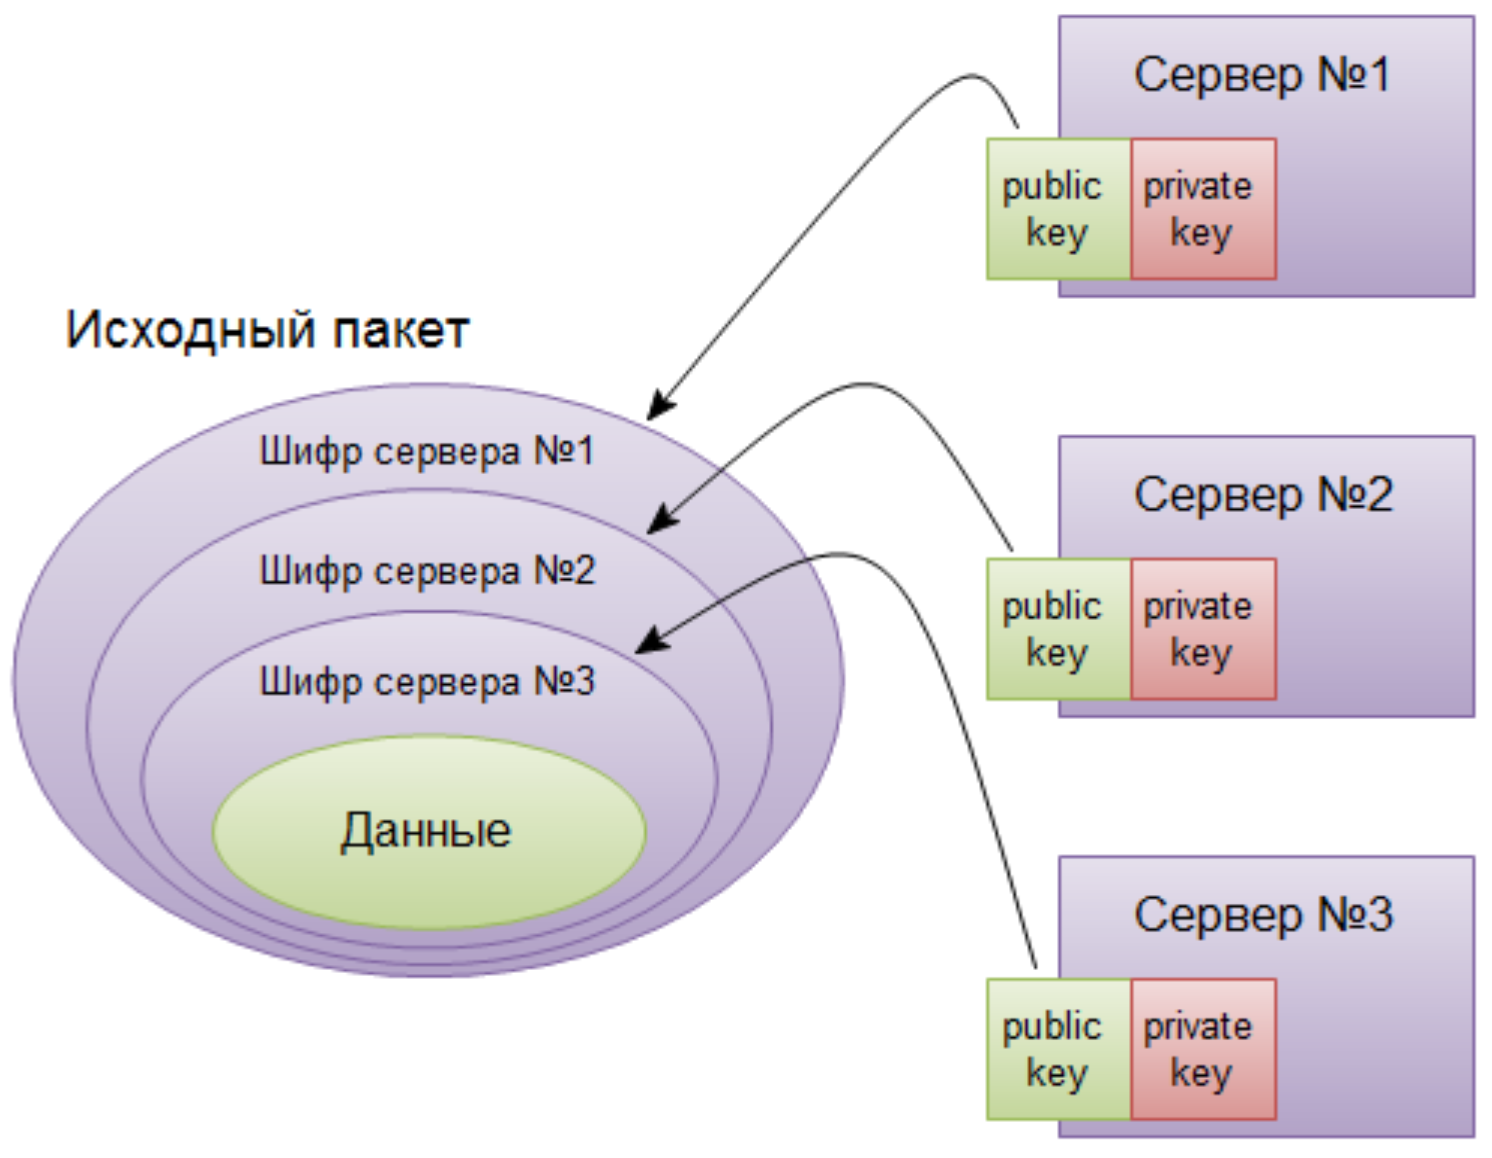
\includegraphics[scale=0.18]{pics/onion-routing.png}
\end{wrapfigure}

Каждый отдельный уровень шифрования дешифруется очередным маршрутизатором. Из дешифрованных данных извлекается адрес следующего маршрутизатора. Сообщение отправляется на следующий маршрутизатор.

\subsubsection{Виды атак на анонимные сети}

\begin{enumerate}
    \item \textit{Атака на кодировку сообщения}. Если сообщение не меняет свое содержимое при прохождении по анонимной сети, весь его маршрут может быть восстановлен
    \item \textit{Атака на длину сообщения}. Если сообщение сохраняет свой размер при передаче по сети, его маршрут может быть восстановлен
    \item \textit{Атака на воспроизведение}. Атакующий может воспроизводить данные ранее переданных сообщений, ожидая, что сеть передаст эти пакеты по тому же маршруту
    \item \textit{Атака путем сговора}. Некоторые участники анонимной сети объединяются для нарушения анонимности остальных участников
    \item \textit{Атака на переполнение}. Переполнение отдельных каналы анонимной сети, чтобы сузить круг пользователей, к которым эти сообщения могут относиться
    \item \textit{Временные атаки}. Оценка продолжительности соединения путем наблюдения фактов установки и окончания соединения в различных точках входа и выхода сети
    \item \textit{Атака на объем данных}. Сопоставление общего объема передаваемых данных в точках входа и выхода сети
    \item \textit{Атака профилирования}. Долговременный анализ соединений некоторого набора пользователей -- обычно комбинация временных атак и атак на объем данных
\end{enumerate}
